\documentclass[11pt]{article}

% Self-contained: compiles with a stock pdflatex/TeX Live install, no external
% conference style files required. To port to the BlackboxNLP/ACL template,
% swap \documentclass for the ACL class and move the title block accordingly.

\usepackage[margin=1in]{geometry}
\usepackage{graphicx}
\usepackage{booktabs}
\usepackage{amsmath}
\usepackage{amssymb}
\usepackage{hyperref}
\usepackage{xcolor}
\usepackage{caption}
\usepackage[numbers,sort&compress]{natbib}
\hypersetup{colorlinks=true, linkcolor=blue!50!black, citecolor=blue!50!black,
            urlcolor=blue!50!black}
\graphicspath{{figures/}}

\title{\textbf{Context Faithfulness Is a Sparse Attention Circuit;\\
Parametric Resistance Is Not: A Controlled Replication and\\
Scale-Boundary Refinement of PH3 in 124M--160M Language Models}}
\author{Rithvik Reddy}
\date{2026}

\begin{document}
\maketitle

\begin{abstract}
When a language model is given retrieved context that contradicts its
parametric memory, which internal components decide whether it defers to the
context or falls back on memory? \citet{jin2024ph3} answer this at the
1.3B--13B scale with two opposing attention-head populations---\emph{context
heads} and \emph{memory heads}---and control the outcome by pruning them
(PH3). We ask whether the same organization holds two orders of magnitude
smaller. Using controlled minimal pairs (a single retrieved number, edited to
agree or disagree with the model's \emph{measured} prior) on GPT-2-small
(124M) and Pythia-160M, we find: (i) context faithfulness is carried by a
sparse, prior-invariant circuit of 2--3 late attention ``mover'' heads that
attend to the retrieved number and copy it into the answer---confirmed by
activation patching, mean-ablation, direct logit attribution, and, crucially,
by PH3's \emph{own} importance metric, under which our movers rank as the top
context heads in both models; but (ii) there is \emph{no functional memory-head
counterpart} at this scale. No head writes the parametric answer or scales its
effect with prior strength. Heads that PH3's importance score flags as
memory-side are, mechanistically, reactive context-\emph{dampeners} that
suppress both answers---a cautionary result for importance-score
interpretation. (iii) Parametric resistance is instead diffuse: a
pre-registered test confirms in Pythia-160M ($\rho=0.37$, one-sided
$p=0.005$, $n=48$ held-out pairs) that resistance appears as a
prior-strength-tracking lean spread across the non-mover attention layer, but
the same test \emph{refutes} it in GPT-2-small ($\rho=0.06$), which we report
as a genuine model split rather than explain away. The study is a controlled
replication that both corroborates PH3's context-head finding and bounds where
its memory-head motif emerges. All code, data, seeds, and a frozen
pre-registration are released.
\end{abstract}

\section{Introduction}

Retrieval-augmented generation places a language model in a recurring bind:
the retrieved context may contradict what the model already ``believes.''
Whether the model trusts the evidence or its own parameters is a faithfulness
question with direct safety and reliability stakes, and it has a mechanistic
answer inside the network. \citet{jin2024ph3} give such an answer for models
from 1.3B to 13B parameters: they localize \emph{context heads} and
\emph{memory heads} with opposing roles via path patching, and show that
pruning one population predictably shifts the model toward the other
knowledge source (their PH3 method raises internal-memory reliance by 44.0\%
and external-context reliance by 38.5\%).

Two questions motivate this work. First, \textbf{does the two-population
picture hold at small scale?} Mechanistic-interpretability tooling
(activation patching, ablation, direct logit attribution) is cheapest and
cleanest on GPT-2-small and Pythia-160M, the field-standard small models, and
a positive result there would make the phenomenon far more tractable to study.
Second, \textbf{is ``defer to good context'' the same circuit as ``resist bad
context,'' or two circuits?} If resistance is a distinct, prior-tracking head
population, that is a strong and localizable claim; if not, the picture is
different from PH3's.

We answer both with a controlled minimal-pair design and a five-phase
protocol in which each phase's verdict was reviewed before the next was built,
and the one confirmatory correlation was \emph{pre-registered} against a
committed git hash before the held-out data existed. Our contributions:

\begin{itemize}
\item A \textbf{sparse, prior-invariant context circuit} in both models
(GPT-2-small heads \texttt{L9H9}, \texttt{L10H2}; Pythia-160M \texttt{L8H10},
\texttt{L10H7}, \texttt{L8H2}), established by four independent methods and
robust to metric choice---it is the top of PH3's context-head ranking too.
\item A \textbf{scale boundary}: no functional memory heads at 124M--160M. We
show PH3's importance metric \emph{does} return a memory-side list at this
scale, but that the flagged heads fail every functional test of a memory
head---a caution that importance scores alone can mislabel suppression heads.
\item A \textbf{pre-registered, model-split result on resistance}: in
Pythia-160M parametric resistance is a diffuse ``attention tide'' that scales
with prior strength; in GPT-2-small the same test fails. We report the split
honestly.
\item A negative result: negation-based context edits produce no usable signal
at this scale, in contrast to numeric edits.
\end{itemize}

We frame this explicitly as a controlled replication and refinement of PH3,
not a first mechanistic account of knowledge conflict.

\section{Method}
\label{sec:method}

\paragraph{Minimal pairs.} Each item is one question plus a short retrieved
``context'' passage stating a single fact, rendered as
\texttt{Context: \{context\}\textbackslash n\textbackslash nQuestion:
\{question\}\textbackslash nAnswer:}. Two versions differ by exactly one
token---the critical number---so that a supportive context states the answer
the model already prefers and a conflicting context states the alternative.
Both candidate answers are single tokens in both tokenizers; the two prompts
tokenize to equal length differing at one position. We use numeric facts
(ages of majority, notice periods, statutory counts, and disjoint world/count
facts) because a pilot showed that negation edits produce no measurable
conflict at this scale (Section~\ref{sec:pilot}).

\paragraph{Measured-prior anchoring.} We do not assume which answer the model
``believes.'' For every candidate we probe the bare prior---the model's
next-token preference between the two answers given the question alone, no
context---and define the winner as the parametric answer and the loser as what
the conflicting context asserts. A pilot found our \emph{a priori} guesses
about the models' beliefs were wrong roughly half the time, so this
measurement is load-bearing. Pairs enter the study only if the measured prior
exceeds a small threshold ($|\Delta\text{logit}|\ge 0.5$) and the context edit
moves behavior by at least one logit (denominator gate).

\paragraph{Behavioral metric.} Throughout we read a logit difference at the
final position, $\mathrm{LD} = \text{logit}(a_\text{context}) -
\text{logit}(a_\text{prior})$: positive means the model follows the
(conflicting) context. This continuous, field-standard readout is more
sensitive than accuracy.

\paragraph{Causal and attributive tools.} We use bidirectional activation
patching (denoising and noising) over the residual stream, attention/MLP
outputs, and individual attention heads; mean-ablation of heads and MLP layers
(mean, not zero, to stay on-distribution, following
\citealp{heimersheim2024patching}); direct logit attribution (DLA) with exact
final-LayerNorm scaling, validated to reconstruct the true logit difference to
$<10^{-5}$; and OV-circuit copy scores. Every experiment fixes and logs
seed~0; forward passes over frozen models are deterministic. All computation
is CPU-only, via TransformerLens \citep{nanda2022tl}.

\section{Phase 0: Is the conflict measurable?}
\label{sec:pilot}

Before building any pipeline we tested the single load-bearing assumption:
that a small model shows measurable context-vs-memory conflict at all. On 16
hand-built pairs, editing one number in the context produced a mean logit
shift of $-3.9$ (GPT-2) / $-3.7$ (Pythia) toward the context answer, with all
8 numeric pairs shifting in the expected direction in both models (sign-test
$p=0.008$). Residual preference under conflicting context tracked the measured
prior at $r\approx0.95$, and the strongest priors resisted the edit---genuine
conflict, not mere copying. Negation edits (``has the right'' vs. ``does not
have the right'') produced no usable signal ($|\text{shift}|\le0.35$,
wrong-signed cases, a uniform token bias), and are dropped. We proceed with
numeric edits only.

\section{Phase 1: A sparse context circuit}
\label{sec:phase1}

We built $\sim$30 measured-prior-anchored pairs per model and ran the full
patching grid. Restoring the conflicting-context activation of the critical
number recovers the override at the number's own position through
$\sim$three-quarters depth, then the signal appears at the answer position in
the last layers---a direct attention hop, not a relay. Head-level patching
localizes the hop to \textbf{2--3 late heads}: GPT-2 \texttt{L9H9} (normalized
recovery 0.47) and \texttt{L10H2} (0.37), together $\approx$84\% of the
head-level effect; Pythia \texttt{L8H10} (0.51), \texttt{L10H7} (0.25),
\texttt{L8H2} (0.15), $\approx$92\% (Figure~\ref{fig:heads}). Denoising and
noising agree. Splitting pairs by prior strength, the same heads top both
terciles (overlap@10 $=$ 90--100\% for GPT-2), a first indication that the
context circuit is invariant to how strongly the prior is held.

\begin{figure}[t]
\centering
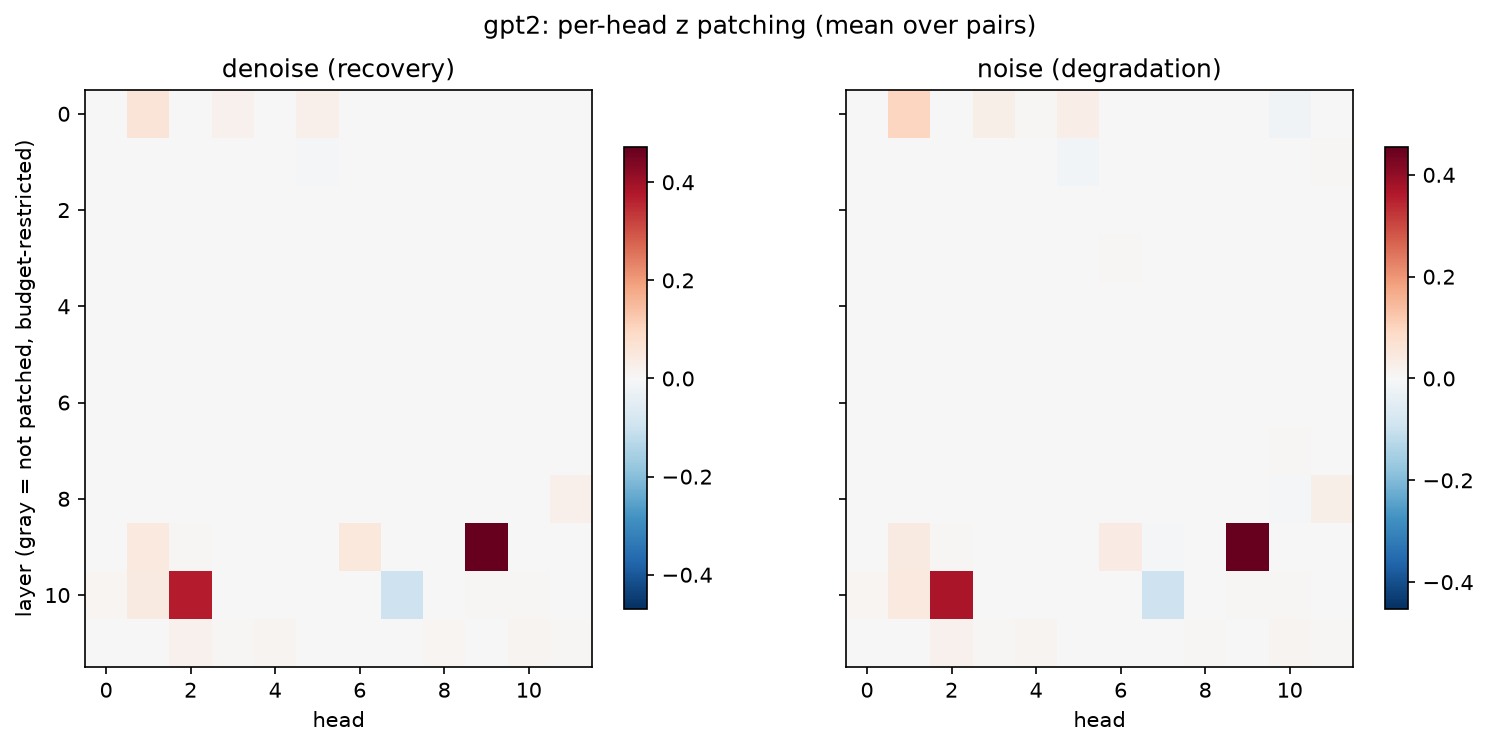
\includegraphics[width=0.49\linewidth]{phase1_heads_gpt2.png}
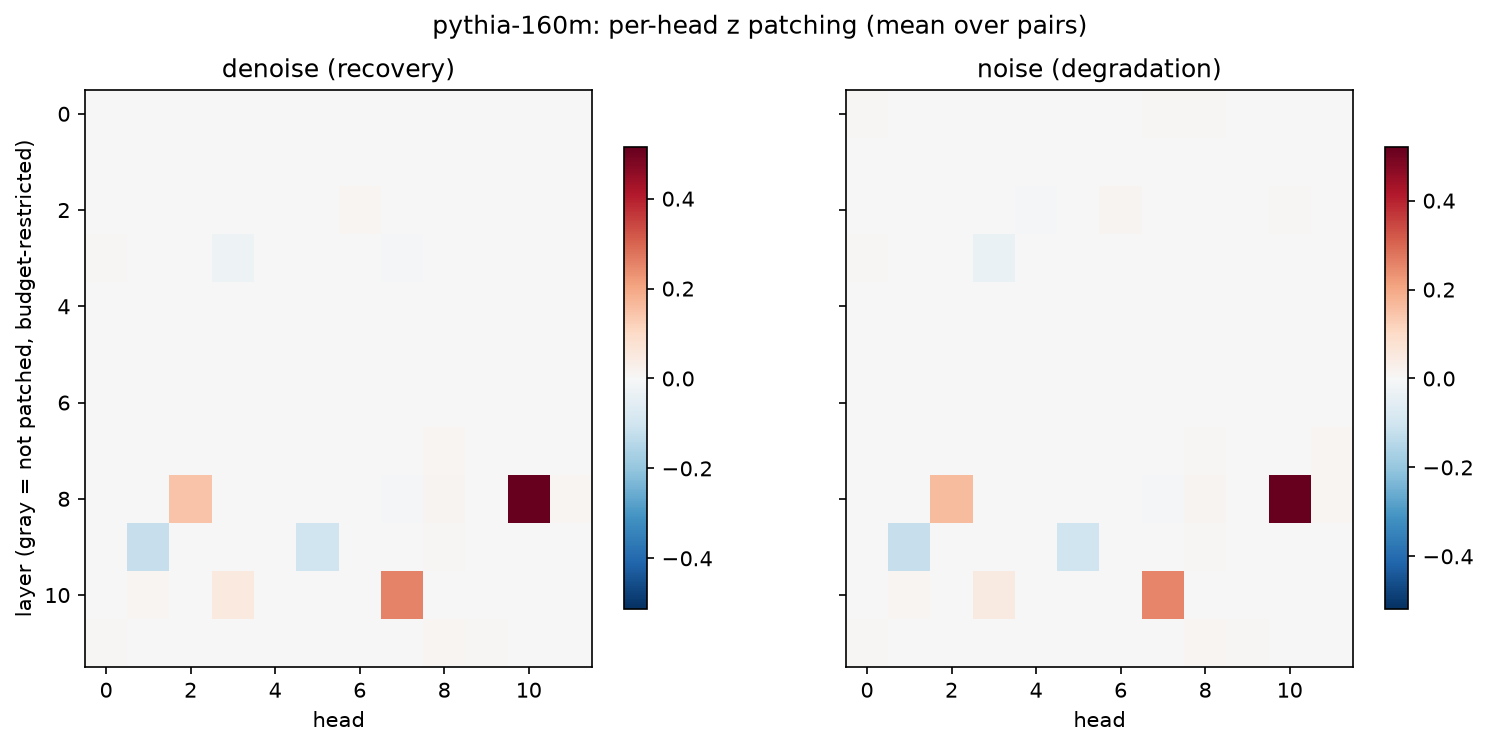
\includegraphics[width=0.49\linewidth]{phase1_heads_pythia-160m.png}
\caption{Per-head activation-patching effect (denoising and noising) at the
answer position. A sparse set of late heads dominates in each model; gray
cells were not patched under the compute budget. See
Section~\ref{sec:phase1}.}
\label{fig:heads}
\end{figure}

\section{Phase 2: The circuit is necessary, and it is a copy mechanism}
\label{sec:phase2}

Mean-ablating the mover heads collapses context-following: GPT-2
\texttt{L9H9+L10H2} drops the context-following rate from 0.97 to 0.27
($\Delta\mathrm{LD}=-1.47$); Pythia's three movers drop it from 0.75 to 0.09
($\Delta\mathrm{LD}=-1.53$); five random near-zero heads sit at the noise floor
($|\Delta\mathrm{LD}|<0.03$) (Figure~\ref{fig:ablation}). In the supportive
condition, where context agrees with the prior, the same ablation moves logits
toward the (shared) answer without breaking context-following---a specificity
signature: the head writes \emph{whatever the context states}.

Attribution turns ``mover head'' into a mechanism. Every mover attends from the
answer position to the retrieved number (GPT-2 \texttt{L9H9} 0.50,
\texttt{L10H2} 0.39; Pythia \texttt{L8H10} 0.65, \texttt{L10H7} 0.99,
\texttt{L8H2} 0.73), writes the context direction (all DLA positive, $+0.20$ to
$+0.80$), and---for the strongest---has an OV circuit that copies the number
token to its own logit (top-vocab percentiles 93--99.9). Single-head ablation
shows no backup-head compensation of the kind reported for name-mover heads in
the IOI circuit \citep{wang2023ioi}, though it cannot rule out joint redundancy
among untested subsets.
This phase also surfaced \emph{negative} heads that write against the context
answer; ablating them \emph{raises} context-following. We return to them in
Phase 3.

\begin{figure}[t]
\centering
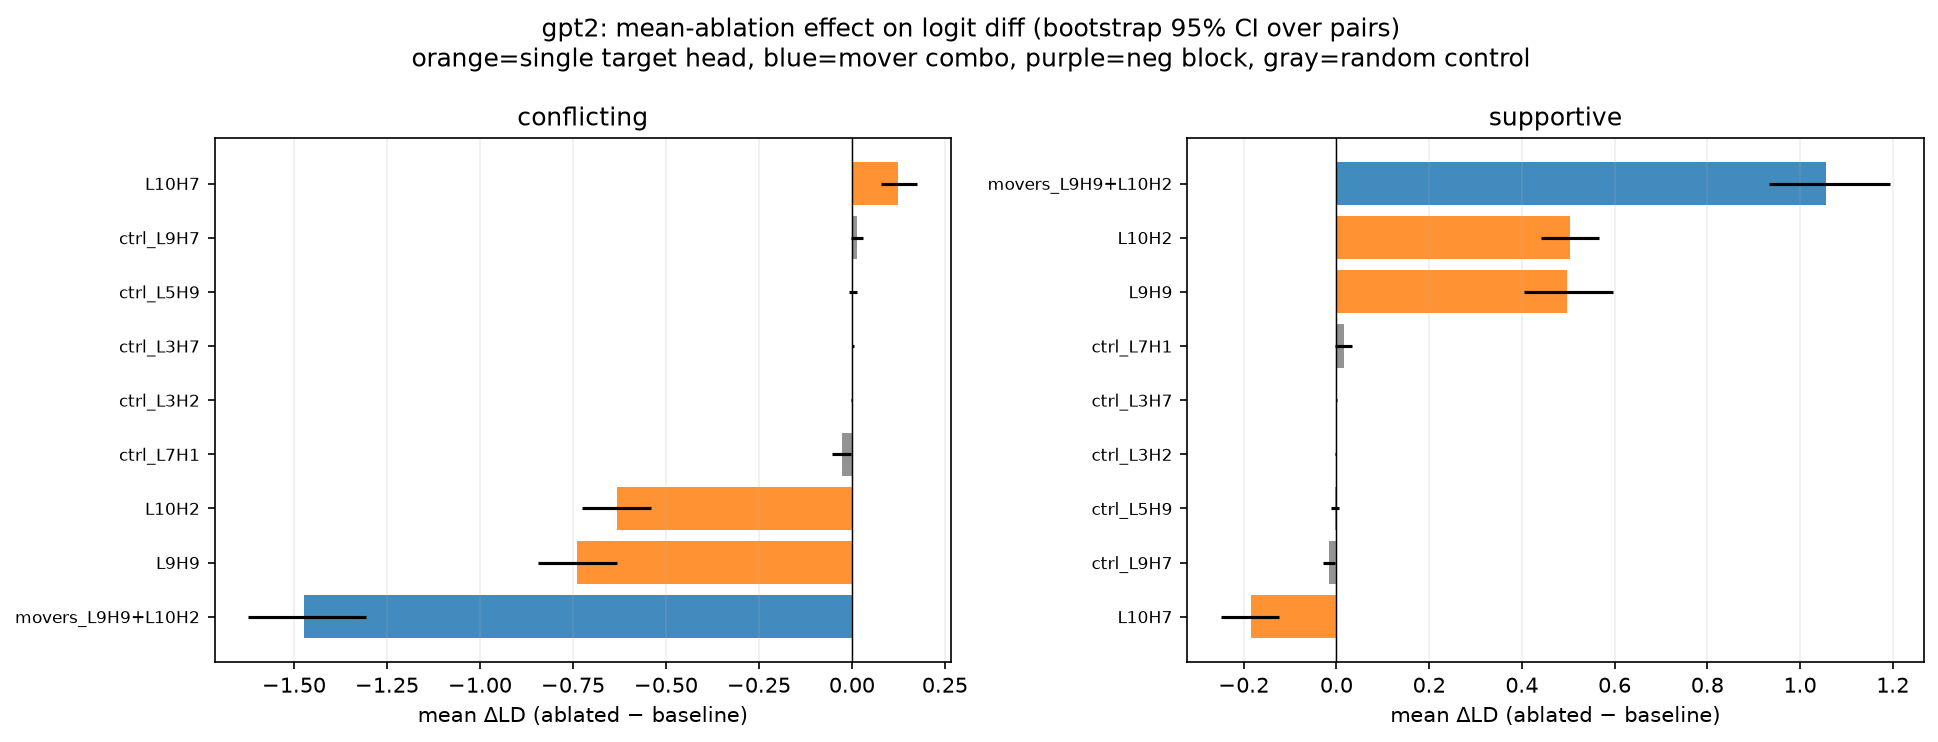
\includegraphics[width=0.49\linewidth]{phase2_ablation_gpt2.png}
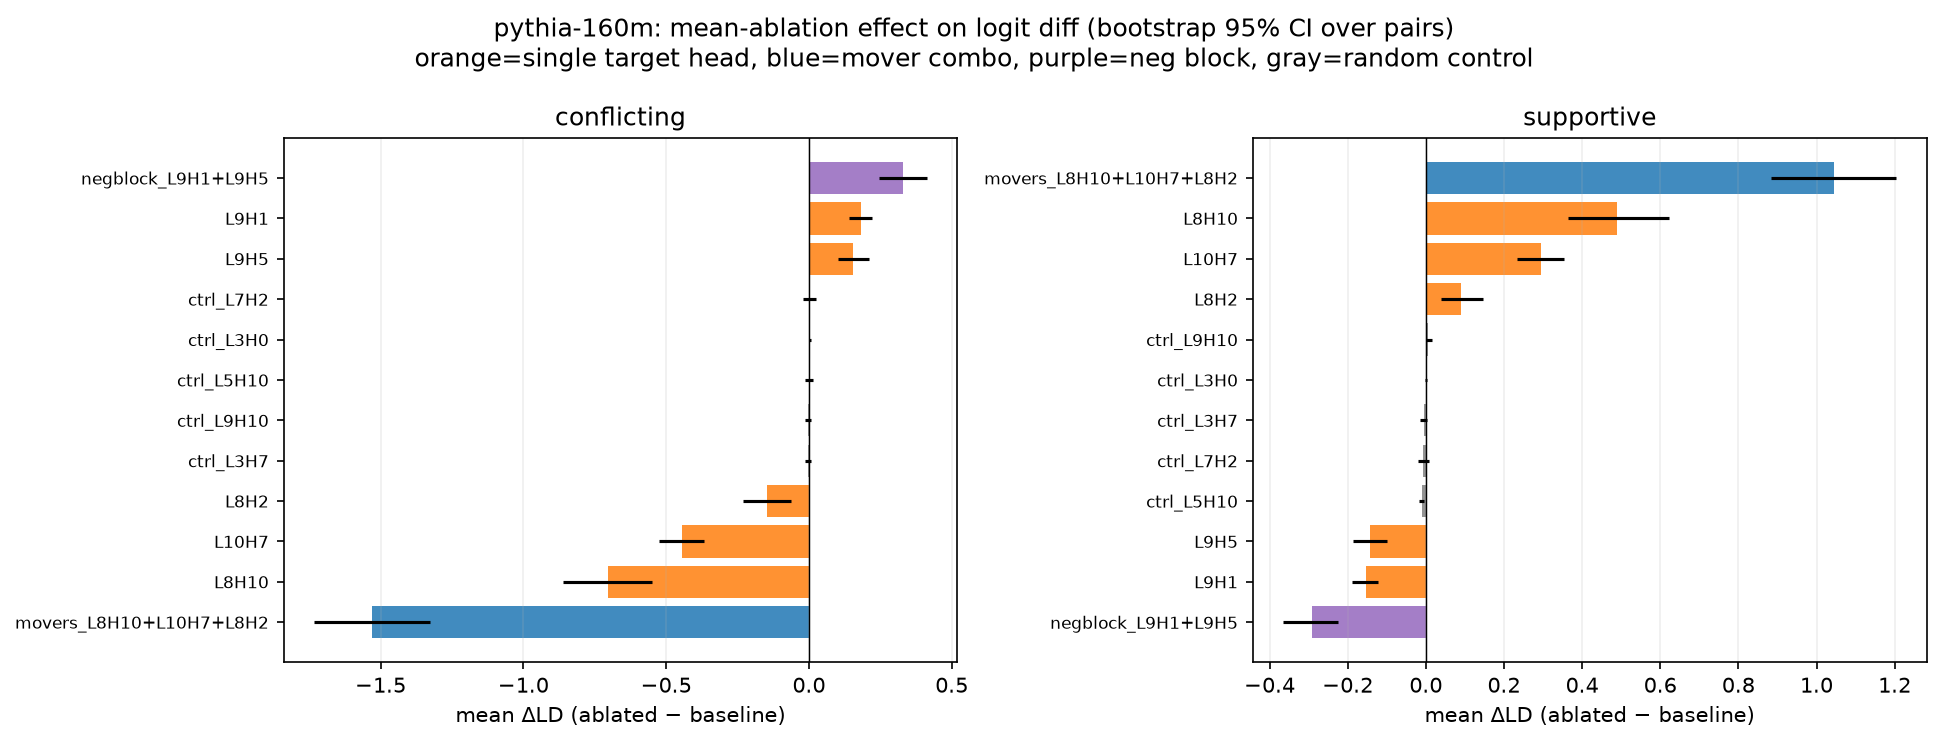
\includegraphics[width=0.49\linewidth]{phase2_ablation_pythia-160m.png}
\caption{Mean-ablation effect on the logit difference (bootstrap 95\% CIs over
pairs). Movers (single and combined) collapse context-following; random
controls are at the noise floor; the negative heads push the other way.}
\label{fig:ablation}
\end{figure}

\section{Phase 3: No memory heads}
\label{sec:phase3}

If resistance were a memory-head population, some head should write the
\emph{prior} answer and matter more when the prior is strong. We test this
directly. Projecting each head's output onto the prior direction and the
context direction separately, the negative heads write \emph{against} both
answers (negative DLA on prior too); they do not carry parametric memory.
Their effect \emph{anti}-scales with prior strength (Pythia $\rho=-0.38$,
$p=0.035$) and vanishes when the movers are ablated first---they are reactive
dampers, not an independent population. Their attention confirms heterogeneity:
Pythia \texttt{L9H1} attends to the answer position itself (a suppression-head
signature), while \texttt{L9H5} and GPT-2 \texttt{L10H7} anti-copy the number
(OV percentiles 11 and 27). A scan over all 144 heads finds the memory-head
region empty in both models: the strongest prior-leaning head reaches only
$+0.10$/$+0.14$ against mover context-leans of $-0.80$/$-0.64$
(Figure~\ref{fig:scan}). The mover circuit, by contrast, is confirmed
prior-invariant a third way (ablation effect vs. prior strength: $\rho=+0.07$
GPT-2, $+0.02$ Pythia).

\begin{figure}[t]
\centering
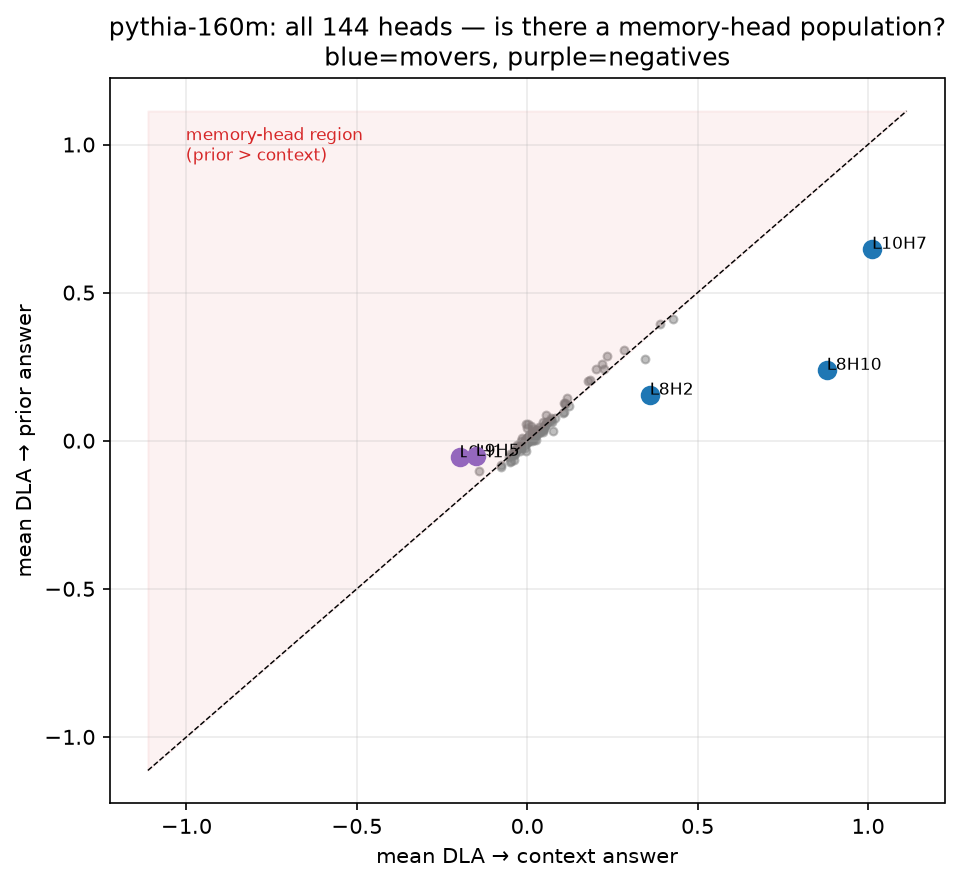
\includegraphics[width=0.62\linewidth]{phase3_scan_pythia-160m.png}
\caption{Direct-logit-attribution scan of all 144 Pythia-160M heads onto the
prior direction ($y$) vs. the context direction ($x$). The memory-head region
(upper-left, prior $>$ context) is empty; the movers (blue) sit far to the
context side. GPT-2 is analogous.}
\label{fig:scan}
\end{figure}

\section{Phase 4: Where resistance lives}
\label{sec:phase4}

If no head carries the prior, what does? Decomposing the answer-position logit
difference into embedding, per-layer attention, and per-layer MLP
contributions refutes the natural guess that MLPs store and inject the memory
answer: MLPs write \emph{both} answers strongly but net-lean toward
\emph{context}, and mean-ablating the top prior-writing MLP layers
\emph{reduces} context-following ($\Delta\mathrm{LD}=-0.46$ GPT-2, $-0.45$
Pythia)---late MLPs are shared amplification, not memory. Instead, the
prior-tracking signal is a diffuse lean across the \emph{non-mover attention}
layer: it flips to the prior side exactly on the pairs where context loses
(Figure~\ref{fig:resistance}) and, in an exploratory analysis, correlates with
prior strength (Pythia $\rho=+0.46$). Because that analysis was post-hoc---the
phase's pre-stated predictions had just failed---we did not report it as a
finding until it survived the pre-registered test of Phase 5. We distinguish
storage (facts may still live in MLPs upstream, in the sense of
\citealp{meng2022rome}) from \emph{transport} into the answer logits, which is
what DLA measures and which is attention-side here.

\begin{figure}[t]
\centering
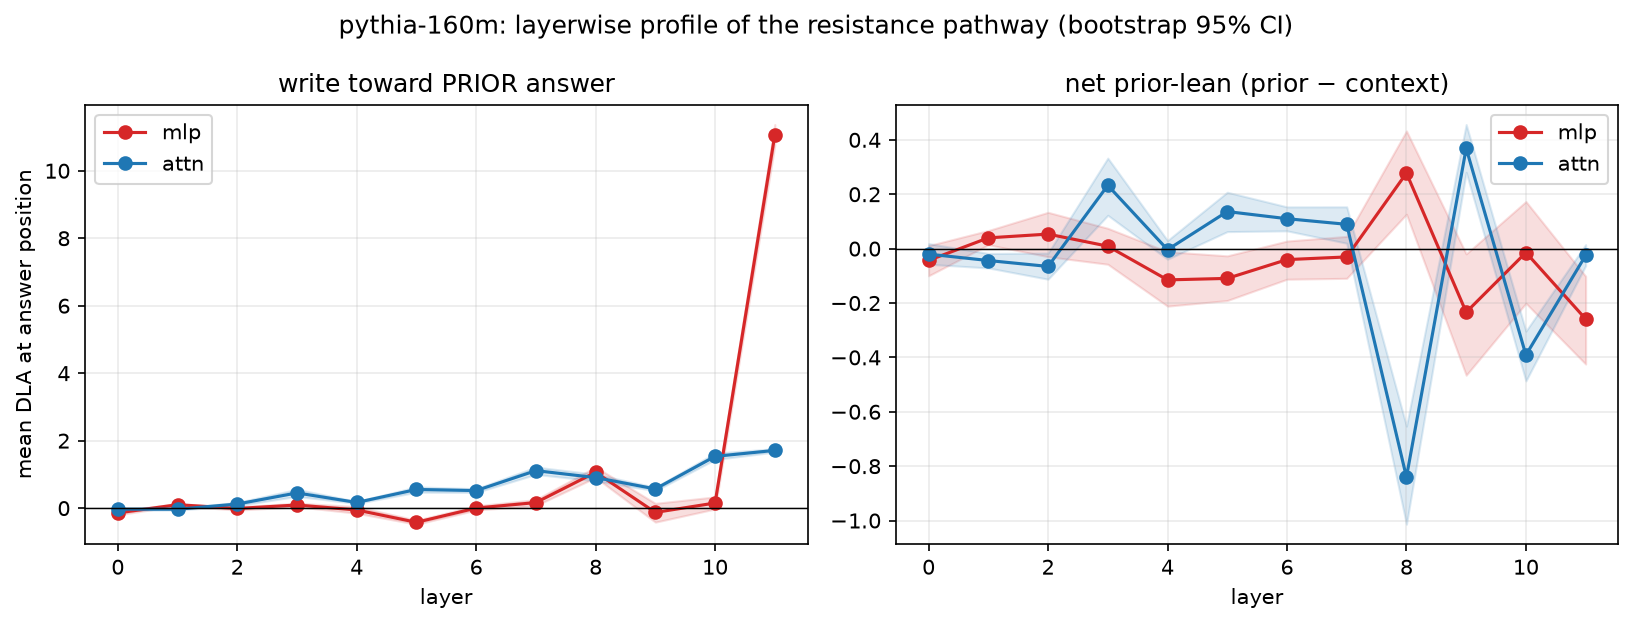
\includegraphics[width=0.49\linewidth]{phase4_layerwise_pythia-160m.png}
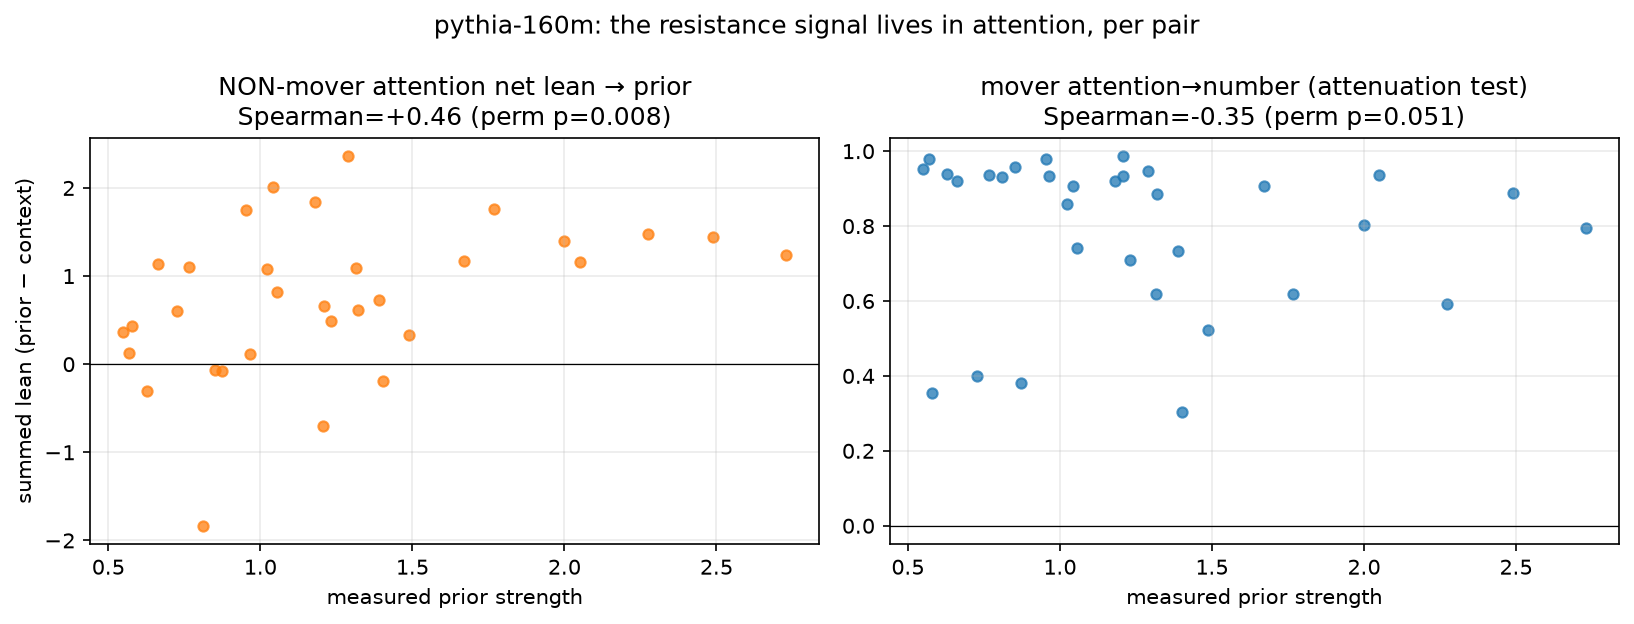
\includegraphics[width=0.49\linewidth]{phase4_resistance_pythia-160m.png}
\caption{Left: layerwise DLA; MLPs do not net-write the prior. Right: the
non-mover attention lean scales with prior strength (exploratory in Phase 4,
pre-registered in Phase 5).}
\label{fig:resistance}
\end{figure}

\section{Phase 5: PH3 metric match and a pre-registered test}
\label{sec:phase5}

\paragraph{PH3's own metric.} We reimplement PH3's head-importance score
(unk-corrupted head patching on the context-minus-memory probability gap; EOS
substitutes for a true \texttt{<unk>}) and rescan all heads. The context side
replicates cleanly: our movers are the top context heads under PH3's metric in
both models (GPT-2 \texttt{L9H9}, \texttt{L10H2} rank 1--2 of 144; Pythia
\texttt{L8H10}, \texttt{L10H7}, \texttt{L8H2} rank 1--3). PH3's metric
\emph{does} return a memory-side top-5\% at this scale---led, in both models,
by exactly our negative heads. But those heads fail every functional test of a
memory head (Phase 3). The correct reading is therefore not ``the region is
empty under all metrics'' but the sharper ``\emph{no head has the memory-head
function at this scale, and importance scores alone can mislabel context
dampeners as memory heads.}'' (Table~\ref{tab:ph3}.)

\paragraph{Pre-registered tide test.} We froze a directional hypothesis with a
specific statistic, thresholds, and decision rule to a committed git hash
(\texttt{539355a}) \emph{before} generating any held-out data, then built a
fresh, fact-disjoint set and ran only that test. In Pythia-160M the tide is
\textbf{confirmed}: Spearman $\rho=+0.368$ between prior strength and non-mover
attention lean, one-sided permutation $p=0.0045$, $n=48$ gated pairs
(Figure~\ref{fig:tide}). In GPT-2-small it is \textbf{refuted}: $\rho=+0.063$,
$p=0.34$. We report the model split as-is; GPT-2's resistance regime is thin
(7 of 48 pairs have context losing, vs.\ 11 for Pythia), and a hypothesis that
only registers where the regime is thick is, for GPT-2, unsupported. Both
secondary (context-loses sign) tests were pre-declared invalid because even a
strong-prior-skewed battery could not reach the pre-registered floor of 20
context-loses pairs---itself a finding: under this format small models
overwhelmingly follow context, and genuine resistance is rare.

\begin{table}[t]
\centering
\small
\caption{Comparison to PH3 \citep{jin2024ph3}.}
\label{tab:ph3}
\begin{tabular}{p{0.20\linewidth}p{0.36\linewidth}p{0.36\linewidth}}
\toprule
 & PH3 (Jin et al. 2024) & This work \\
\midrule
Models & 1.3B--13B (OPT, Pythia, LLaMA-2) & GPT-2-small 124M, Pythia-160M \\
Context heads & top-5\%, middle--late & 2--3 movers; also top of PH3's metric \\
Memory heads & top-5\%; pruning shifts to context & \textbf{no functional memory heads}; PH3's metric flags reactive dampers \\
Prior scaling & not analyzed & movers flat; dampers anti-scale \\
Resistance & second head population & diffuse attention-side lean (Pythia, pre-registered); not established (GPT-2) \\
\bottomrule
\end{tabular}
\end{table}

\begin{figure}[t]
\centering
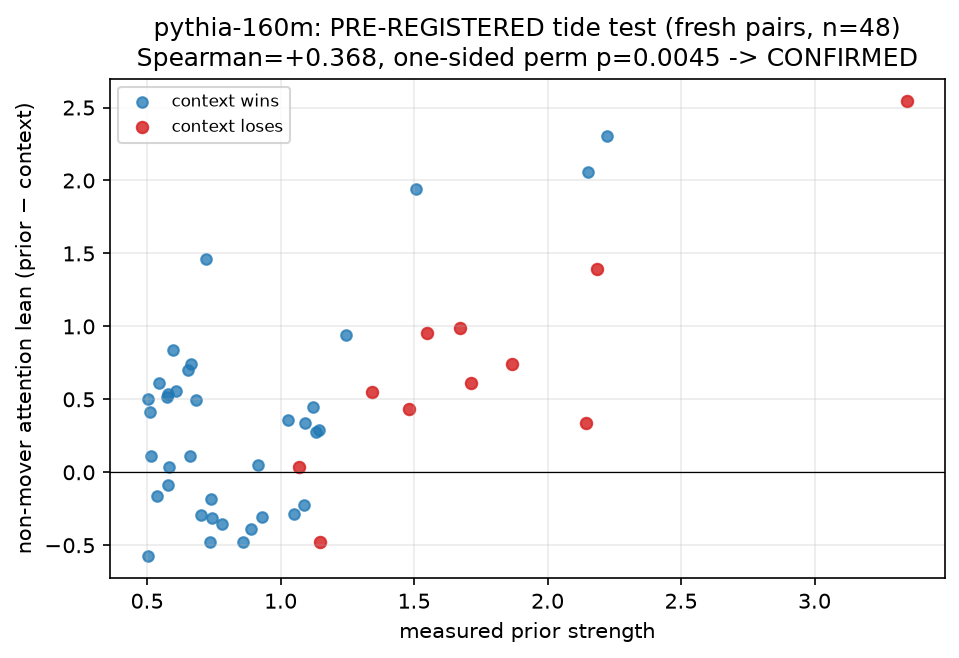
\includegraphics[width=0.49\linewidth]{phase5_tide_pythia-160m.png}
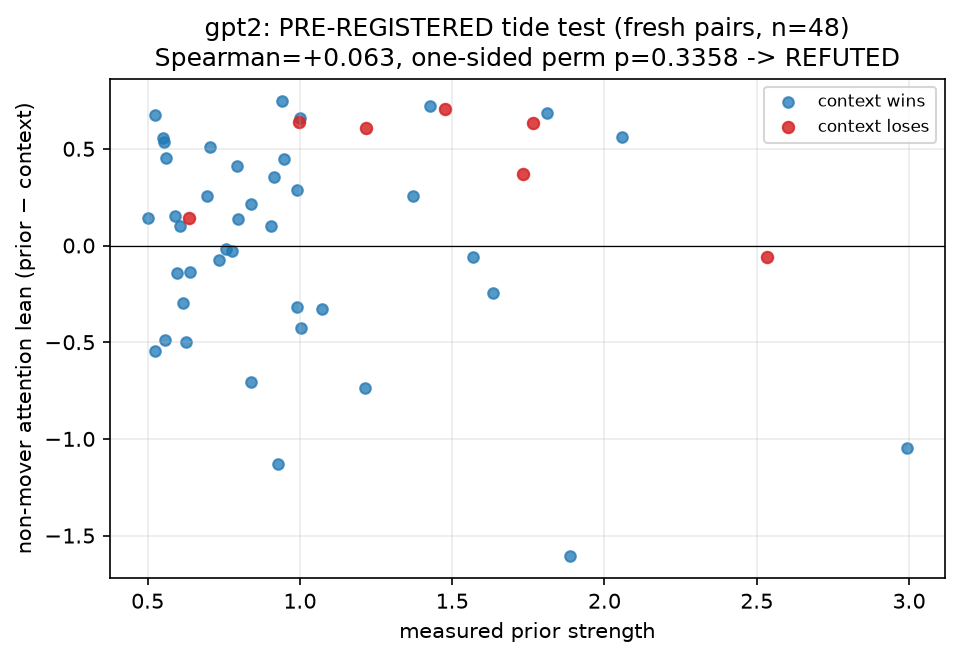
\includegraphics[width=0.49\linewidth]{phase5_tide_gpt2.png}
\caption{Pre-registered tide test on fresh, fact-disjoint pairs. Confirmed in
Pythia-160M (left), refuted in GPT-2-small (right). Red points are pairs where
context loses.}
\label{fig:tide}
\end{figure}

\section{Discussion}

At 124M--160M parameters, faithfulness to retrieved context is a small,
sharply localized, prior-invariant attention circuit that reads a retrieved
fact and copies it to the output---and it is the same circuit PH3's metric
identifies as context heads at billion scale, so the context side of their
picture reaches down two orders of magnitude. The memory side does not. No head
at this scale performs the memory-head function, and the heads an
importance score would label memory-side are suppression/dampening heads that
oppose the movers without carrying the prior. Parametric resistance instead
appears, where it appears at all, as a distributed attention-side lean that
tracks prior strength---confirmed under pre-registration in Pythia-160M and
absent in GPT-2-small. The practical reading: the billion-scale memory-head
motif has an emergence threshold above this range, and dedicated memory heads
are a capability that crystallizes with scale while, at small scale, resistance
stays diffuse.

The methodological takeaway is narrower but sharp: an importance score that
ranks heads by how much patching them changes a context-minus-memory gap will
surface ``memory heads'' even where none carry memory, because suppression
heads move that gap too. Functional tests---does the head write the prior? does
its effect scale with prior strength?---are needed to tell the two apart.

\paragraph{Limitations.} Two models, one prompt template, single-token numeric
answers, and $\le54$ pairs per model bound external validity. DLA attributes to
the final writer, so upstream MLP storage is compatible with attention-side
transport. Our PH3 reimplementation follows the paper's description
(single-dataset variant, EOS for \texttt{<unk>}) but is not their code. The
tide is an aggregate over $\sim$141 heads whose internal structure we do not
resolve. The GPT-2 resistance regime is too thin to test its tide fairly, which
is itself the honest finding rather than a nuisance to be corrected.

\paragraph{Reproducibility.} All code, the minimal-pair sets, per-pair result
tables, figures, fixed seeds, and the frozen pre-registration are released;
every phase regenerates from a clean checkout with a single command on CPU.

\begin{thebibliography}{9}
\bibitem[Jin et al.(2024)]{jin2024ph3}
Zhuoran Jin, Pengfei Cao, Hongbang Yuan, Yubo Chen, Jiexin Xu, Huaijun Li,
Xiaojian Jiang, Kang Liu, and Jun Zhao.
\newblock Cutting off the head ends the conflict: A mechanism for interpreting
and mitigating knowledge conflicts in language models.
\newblock \emph{Findings of ACL}, 2024. arXiv:2402.18154.

\bibitem[Heimersheim and Nanda(2024)]{heimersheim2024patching}
Stefan Heimersheim and Neel Nanda.
\newblock How to use and interpret activation patching.
\newblock arXiv:2404.15255, 2024.

\bibitem[Wang et al.(2023)]{wang2023ioi}
Kevin Wang, Alexandre Variengien, Arthur Conmy, Buck Shlegeris, and Jacob
Steinhardt.
\newblock Interpretability in the wild: a circuit for indirect object
identification in GPT-2 small.
\newblock \emph{ICLR}, 2023.

\bibitem[Meng et al.(2022)]{meng2022rome}
Kevin Meng, David Bau, Alex Andonian, and Yonatan Belinkov.
\newblock Locating and editing factual associations in GPT.
\newblock \emph{NeurIPS}, 2022.

\bibitem[Nanda and Bloom(2022)]{nanda2022tl}
Neel Nanda and Joseph Bloom.
\newblock TransformerLens.
\newblock \url{https://github.com/TransformerLensOrg/TransformerLens}, 2022.
\end{thebibliography}

\end{document}
